\documentclass[11pt]{article}
\usepackage[utf8]{inputenc}
\usepackage[T1]{fontenc}
\usepackage[english]{babel}
\usepackage{amsmath}
\usepackage{amssymb}
\usepackage{geometry}
\usepackage{booktabs}
\usepackage{tabularx}
\usepackage{float}
\usepackage{setspace}
\usepackage{xcolor}
\usepackage{url}
\usepackage{tikz}
\usetikzlibrary{positioning, calc, arrows.meta}
\usepackage[hidelinks]{hyperref}

\geometry{a4paper, margin=1in}
\setstretch{1.25}
\setlength{\emergencystretch}{3em}
\setlength{\parskip}{0.4em}

\newcommand{\R}{\mathbb{R}}
\newcommand{\E}{\mathbb{E}}
\newcommand{\ind}{\mathbf{1}}
\newcommand{\slog}{\operatorname{slog}}
\newcommand{\BCE}{\operatorname{BCE}}
\newcommand{\Huber}{\operatorname{Huber}}
\newcommand{\Bern}{\operatorname{Bernoulli}}
\newcommand{\code}[1]{\texttt{#1}}

\newenvironment{idea}{\begin{quote}\small\color{black!75}\textbf{Key idea.}~}{\end{quote}}

\title{Predicting Behaviour Trajectories with LSTM and GRU\\[0.3em]
\large The theory behind \code{w2\_trajectory\_models.ipynb}}
\author{Workshop 2 · Group 2}
\date{}

\begin{document}
\sloppy
\maketitle

\begin{abstract}
This document collects the theory behind the trajectory notebook of Workshop~2. The goal is no longer to classify whether a user will churn, but to predict what the user will do over the next 7 days: whether they listen, how much they listen, whether they pay, how much they pay and whether they cancel. The model is then used as a simulator for the retention agents in \code{wfinal}. The document explains how the 90-day window is split, what is predicted and why, the recurrent architecture, the composite loss, how full weeks are simulated by predicting events and rebuilding the subscription state, and how everything is evaluated against naive predictors.
\end{abstract}

\tableofcontents
\newpage

% ═════════════════════════════════════════════════════════════════════
\section{From classification to trajectories}
% ═════════════════════════════════════════════════════════════════════

\subsection{What changes}

In the classification notebook (\code{w2\_neural\_models.ipynb}), each user $i$ is represented by a matrix $X_i \in \R^{90 \times 20}$ (90 days, 20 channels) and the model outputs a single number: the churn probability $\hat p_i = P(y_i = 1 \mid X_i)$. It is a \emph{many-to-one} problem: many input steps and one output.

In the trajectory notebook the output is no longer a label but \emph{the user's own future}: a matrix of days by variables. The problem becomes \emph{many-to-many} and, above all, it is no longer pure classification. Some variables are continuous quantities (seconds listened, amount paid) and others are binary events (did they listen?, did they pay?). As shown below, each type of output therefore needs its own activation and its own loss.

\subsection{What it is for}

The agents in \code{wfinal} choose retention actions (reminders, discounts, downgrades, etc.). To train them, an \emph{environment} must answer the question: ``given what this user has done up to today, how will they behave over the next days?''. A trajectory predictor is exactly that: a simulator of the user learned from data.

\subsection{Splitting the window}

The export does not need to be rebuilt. The existing 90-day window is split in two:
\begin{equation}
\underbrace{x_{i,0},\, x_{i,1},\, \dots,\, x_{i,82}}_{\text{input: } T_{\text{in}} = 83 \text{ days}}
\;\Big|\;
\underbrace{x_{i,83},\, \dots,\, x_{i,89}}_{\text{target: } H = 7 \text{ days}} .
\end{equation}

\begin{figure}[H]
\centering
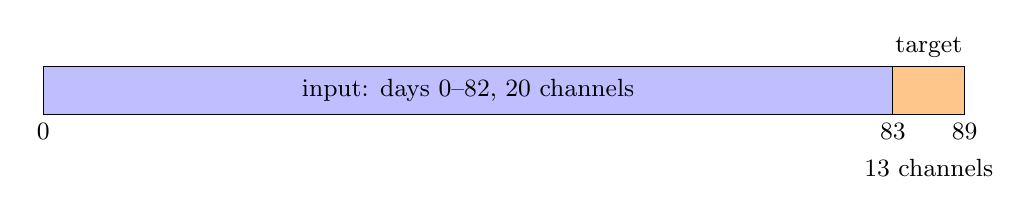
\begin{tikzpicture}[x=0.13cm, y=1cm, font=\small]
  \fill[blue!25] (0,0) rectangle (83,0.6);
  \fill[orange!45] (83,0) rectangle (90,0.6);
  \draw (0,0) rectangle (90,0.6);
  \draw (83,0) -- (83,0.6);
  \node[below] at (0,0) {0};
  \node[below] at (83,0) {83};
  \node[below] at (90,0) {89};
  \node at (41.5,0.3) {input: days 0--82, 20 channels};
  \node[above] at (86.5,0.6) {target};
  \node[below=0.45cm] at (86.5,0) {13 channels};
\end{tikzpicture}
\caption{The 90-day window split into input and target.}
\end{figure}

\begin{table}[H]
\centering
\begin{tabular}{lll}
\toprule
\textbf{Cohort} & \textbf{Input} & \textbf{Target} \\
\midrule
\code{train\_feb} & 2016-11-03 to 2017-01-24 & 2017-01-25 to 2017-01-31 \\
\code{test} (March) & 2016-12-01 to 2017-02-21 & 2017-02-22 to 2017-02-28 \\
\bottomrule
\end{tabular}
\caption{Input and target dates of each cohort.}
\end{table}

The target days are ``future'' relative to what the model sees, not relative to the calendar. This is not a problem because the model never receives the date: it only sees a sequence of 83 days and learns to continue it. As a result, in the environment it can be given the last 83 days before the cutoff and it predicts the following week (Section~\ref{sec:use}).

\subsection{Why $H = 7$}

\begin{itemize}
  \item One week covers a full listening cycle (weekdays and weekend).
  \item The input stays long: 83 days hold almost three months of history.
  \item Daily listening is very noisy. With a longer horizon, almost all of the error would be unpredictable noise and the input would shrink.
  \item One agent turn maps naturally onto one week: action $\to$ 7 simulated days $\to$ new state.
\end{itemize}

% ═════════════════════════════════════════════════════════════════════
\section{The data}
% ═════════════════════════════════════════════════════════════════════

\subsection{The 20 channels}

Each day $t$ of user $i$ is a vector $x_{i,t} \in \R^{20}$ with three blocks:

\begin{itemize}
  \item \textbf{Listening (0--7).} Seven counters (\code{num\_25}, \code{num\_50}, \code{num\_75}, \code{num\_985}, \code{num\_100}, \code{num\_unq}, \code{total\_secs}) and the \code{active} flag, which is 1 if a listening record exists for that day.
  \item \textbf{Payment events (8--12).} \code{tx\_count}, \code{tx\_paid\_sum}, \code{tx\_plan\_days\_sum}, \code{tx\_cancel\_count}, \code{tx\_auto\_renew\_count}. They are non-zero only on days with at least one payment.
  \item \textbf{Subscription state (13--19).} \code{tx\_state\_known}, \code{tx\_last\_is\_cancel}, \code{tx\_last\_is\_auto\_renew}, \code{tx\_days\_since\_last}, \code{tx\_days\_to\_expire}, \code{tx\_expiry\_known}, \code{tx\_state\_ambiguous}. They describe the subscription at the end of each day and are carried forward until the next payment.
\end{itemize}

\subsection{Export encoding}

Quantities have very long tails (a user may listen for 100 seconds or for 50{,}000 seconds in a day). To compress them, the export stores
\begin{align}
&\log(1 + v) && \text{for non-negative quantities}, \\
&\slog(v) = \operatorname{sign}(v)\,\log(1 + |v|) && \text{for quantities that can be negative}.
\end{align}
The signed logarithm is used for \code{tx\_paid\_sum} (negative amounts exist) and \code{tx\_days\_to\_expire} (negative once the membership has expired). Both transformations are invertible:
\begin{equation}
v = e^{u} - 1 = \operatorname{expm1}(u), \qquad v = \operatorname{sign}(u)\,\big(e^{|u|} - 1\big).
\end{equation}
All evaluation is done in this encoding, or after undoing it, never in the scaled space.

\subsection{Masked standard scaling}

Before entering the network, each numeric channel is clipped at an upper quantile and standardised:
\begin{equation}
\tilde x_{i,t,k} =
\begin{cases}
\dfrac{\min(x_{i,t,k},\, u_k) - \mu_k}{\sigma_k} & \text{if the channel is defined on that day,} \\[0.8em]
0 & \text{otherwise.}
\end{cases}
\end{equation}
The mean $\mu_k$ and standard deviation $\sigma_k$ are computed \emph{only on the days where the channel is defined}: active days for listening, payment days for events and days with a known state for states. The parameters are fitted on \code{fit} during the search and on all of February (\code{development}) for the final model. Binary flags are not scaled.

\begin{idea}
After scaling, an inactive day is 0 and an \emph{average} active day is also 0. In the scaled space, ``did not listen'' and ``listened as usual'' are the same number. This coincidence is the underlying reason for the hurdle model of Section~\ref{sec:hurdle}.
\end{idea}

\subsection{The 13 targets}

For each user the target is a tensor $Y_i \in \R^{7 \times 13}$:

\begin{table}[H]
\centering
\renewcommand{\arraystretch}{1.2}
\begin{tabularx}{\textwidth}{clXl}
\toprule
\textbf{Pos.} & \textbf{Target} & \textbf{What it is} & \textbf{Defined on} \\
\midrule
0--6 & listening & the 7 counters, scaled & active days \\
7 & \code{active} & $\ind[\text{listening record exists}]$ & every day \\
8 & \code{pay} & $\ind[\code{tx\_count} > 0]$ & every day \\
9--10 & amount and plan & \code{tx\_paid\_sum}, \code{tx\_plan\_days\_sum}, scaled & payment days \\
11 & \code{cancel} & $\ind[\code{tx\_cancel\_count} > 0]$ & payment days \\
12 & \code{auto\_renew} & $\ind[\code{tx\_auto\_renew\_count} > 0]$ & payment days \\
\bottomrule
\end{tabularx}
\caption{Layout of the target $Y_i \in \R^{7 \times 13}$.}
\end{table}

Binary targets are read from the \emph{unscaled} tensor. For example, a day with one payment has $\code{tx\_count} = \log 2 \approx 0.693$ in the export. With the mean and standard deviation of \code{fit} ($\mu \approx 0.697$, $\sigma \approx 0.037$) this becomes $(0.693 - 0.697)/0.037 \approx -0.1$. Reading the scaled value would encode ``paid'' as $-0.1$ instead of 1.

The 7 state channels are \emph{not} targets. Section~\ref{sec:states} explains why.

% ═════════════════════════════════════════════════════════════════════
\section{Events and states}
\label{sec:states}
% ═════════════════════════════════════════════════════════════════════

\subsection{States are arithmetic on events}

Once the events of a day are known, the state of the next day is fully determined:
\begin{itemize}
  \item With a payment: \code{days\_since\_last} goes back to 0, the flags take the values of the payment and the expiry moves.
  \item Without a payment: \code{days\_since\_last} increases by 1 and \code{days\_to\_expire} decreases by 1.
\end{itemize}
The state carries no new information: it is a deterministic function of the events and the previous state.

\subsection{Predict events, rebuild states}

The network therefore predicts only the 13 event targets. To simulate a week, one concrete scenario is \emph{sampled} from the predicted probabilities (the user pays or does not pay), and the state is computed with the same rules as the export (Section~\ref{sec:simulation}). Two properties follow:

\begin{itemize}
  \item \textbf{Coherence by construction.} A simulated payment always resets \code{days\_since\_last} and moves the expiry; no trajectory can contradict itself.
  \item \textbf{Only possible values.} Every simulated day is a state that a real user could be in, never an average of several futures.
\end{itemize}

\begin{idea}
The simulator produces \emph{one possible future} per user, not the average of the possible futures. An environment needs exactly that, because it must be able to move forward through valid states.
\end{idea}

\subsection{Fit with the environment}

In \code{wfinal}, the customer is stored as raw data (transactions and logs) and the \code{SequenceBuilder} recomputes the states from the payments. Simulated events fit directly into that representation: they are payments and listening days.

% ═════════════════════════════════════════════════════════════════════
\section{The model}
% ═════════════════════════════════════════════════════════════════════

\subsection{Recurrent encoder}

The network reads the 83 days in order and keeps a hidden state $h_t \in \R^{H_d}$ that summarises everything seen up to day $t$. Two cells are compared.

\paragraph{LSTM.} It uses a separate memory $c_t$ and three gates:
\begin{align}
f_t &= \sigma(W_f x_t + U_f h_{t-1} + b_f) && \text{(forget)} \\
i_t &= \sigma(W_i x_t + U_i h_{t-1} + b_i) && \text{(input)} \\
o_t &= \sigma(W_o x_t + U_o h_{t-1} + b_o) && \text{(output)} \\
\tilde c_t &= \tanh(W_c x_t + U_c h_{t-1} + b_c) \\
c_t &= f_t \odot c_{t-1} + i_t \odot \tilde c_t \\
h_t &= o_t \odot \tanh(c_t).
\end{align}
The additive update of $c_t$ lets the gradient travel through many steps without vanishing: if $f_t \approx 1$, the memory passes almost unchanged. Each layer has four weight blocks.

\paragraph{GRU.} It merges memory and hidden state into a single vector:
\begin{align}
r_t &= \sigma(W_r x_t + U_r h_{t-1} + b_r) && \text{(reset)} \\
u_t &= \sigma(W_u x_t + U_u h_{t-1} + b_u) && \text{(update)} \\
n_t &= \tanh\!\big(W_n x_t + b_n + r_t \odot (U_n h_{t-1} + d_n)\big) \\
h_t &= (1 - u_t) \odot n_t + u_t \odot h_{t-1}.
\end{align}
When $u_t \approx 1$ it keeps its memory; when $u_t \approx 0$ it replaces it with the candidate. It uses three weight blocks instead of four, so it is smaller and faster for the same hidden size.

\paragraph{Stacking.} Two or three layers are stacked: the first reads the 20 channels and each following layer reads the hidden states of the one below. Initial states are zero.

\subsection{User summary and normalisation}

After day 82 (the last input day), the top layer outputs $h_{83} \in \R^{H_d}$: a learned summary of the user's whole behaviour. It is normalised with \code{BatchNorm1d}:
\begin{equation}
\tilde h = \gamma \odot \frac{h_{83} - \mu_B}{\sqrt{\sigma^2_B + \epsilon}} + \beta,
\end{equation}
where $\mu_B$ and $\sigma^2_B$ are the batch mean and variance and $\gamma$, $\beta$ are learned parameters. This stabilises the scale of the input to the head and makes training easier.

\subsection{Direct multi-horizon head}

The head is a single linear layer that emits all 7 days at once:
\begin{equation}
z = W \tilde h + b \in \R^{91}, \qquad Z = \operatorname{reshape}(z) \in \R^{7 \times 13}.
\end{equation}
$Z_{h,j}$ is the output for day $83 + h - 1$ and target $j$. The 6 binary positions are \emph{logits} (the sigmoid is applied inside the loss or at prediction time) and the 7 quantity positions are scaled values.

\begin{figure}[H]
\centering
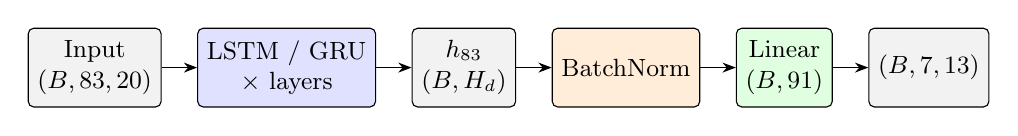
\begin{tikzpicture}[
  box/.style={draw, rounded corners=2pt, minimum height=1.0cm, align=center, font=\small, fill=#1},
  box/.default={gray!10}, >=Stealth, node distance=0.45cm]
  \node[box] (in) {Input\\$(B, 83, 20)$};
  \node[box=blue!12, right=of in] (rnn) {LSTM / GRU\\$\times$ layers};
  \node[box, right=of rnn] (h) {$h_{83}$\\$(B, H_d)$};
  \node[box=orange!15, right=of h] (bn) {BatchNorm};
  \node[box=green!12, right=of bn] (fc) {Linear\\$(B, 91)$};
  \node[box, right=of fc] (out) {$(B, 7, 13)$};
  \draw[->] (in) -- (rnn); \draw[->] (rnn) -- (h); \draw[->] (h) -- (bn);
  \draw[->] (bn) -- (fc); \draw[->] (fc) -- (out);
\end{tikzpicture}
\caption{Architecture shared by LSTM and GRU. Only the recurrent cell changes.}
\end{figure}

\paragraph{Why not an autoregressive decoder?} The alternative would be to predict day 83, feed it back as input, predict day 84, and so on. It has two drawbacks:
\begin{enumerate}
  \item \textbf{Error accumulation:} each day is predicted from days that were already predicted, so errors chain together.
  \item \textbf{It would need all 20 channels at every step}, including the states, to feed them back.
\end{enumerate}
With a horizon of only 7 days, the direct head is simpler and sufficient. Chaining is done in blocks of one week (Section~\ref{sec:rollout}), where the states are rebuilt correctly.

\subsection{Capacity}

In the classifier the smallest configuration won (32 units, 2 layers), but there the network had to produce a single number. Now the vector $\tilde h$ must encode 91 outputs, so the search space is widened to $H_d \in \{64, 128, 256\}$.

% ═════════════════════════════════════════════════════════════════════
\section{Hurdle model for listening}
\label{sec:hurdle}
% ═════════════════════════════════════════════════════════════════════

\subsection{The problem of zeros}

Daily listening has a large mass at zero (days without listening) and a continuous part (days with listening). If a single regression is fitted over all days, for a user who listens with probability $p$ and, when listening, about $m$ (in $\log 1p$), the optimal prediction under squared loss is
\begin{equation}
\E[Y] = p \cdot m + (1 - p) \cdot 0 = p\,m.
\end{equation}
With $p = 0.5$ and $m = 9$ (about 8{,}000 seconds), the model predicts $4.5$ (about 90 seconds) \emph{every day}. That user does not exist: the real one listens a lot on some days and not at all on others. Moreover, since in the scaled space zero coincides with the average active day, the model can reach a low error by predicting almost zero everywhere without learning anything.

\subsection{Two-part decomposition}

The hurdle model separates the two questions:
\begin{equation}
Y = A \cdot M, \qquad A \sim \Bern(\pi), \qquad M \mid A = 1 \sim \text{distribution of the amount}.
\end{equation}
\begin{itemize}
  \item $\pi = P(\text{active})$ is learned with binary cross-entropy on \code{active}.
  \item The amount is learned with the Huber loss \emph{on active days only}.
\end{itemize}
When a point forecast is needed (for the MAE), the model uses
\begin{equation}
\hat y = \hat\pi \cdot \hat m .
\end{equation}
When simulating, $A$ is sampled and, if it is 1, $\hat m$ is written. This yields days with and without listening, as in the real data.

The same logic applies to payments: \code{pay} is the hurdle, and the amount, plan, cancellation and auto-renewal are learned only on payment days. If the amount were learned on every day, since there is almost never a payment, the model would learn to predict almost zero.

% ═════════════════════════════════════════════════════════════════════
\section{The composite loss}
% ═════════════════════════════════════════════════════════════════════

\subsection{Binary cross-entropy}

For a binary target $y \in \{0, 1\}$ and a logit $z$, with $\hat p = \sigma(z)$:
\begin{equation}
\BCE(z, y) = -\big[y \log \sigma(z) + (1 - y)\log(1 - \sigma(z))\big].
\end{equation}
Its derivative with respect to the logit is simply $\partial \BCE / \partial z = \sigma(z) - y$. PyTorch computes it together with the sigmoid (\code{binary\_cross\_entropy\_with\_logits}), which avoids evaluating $\log 0$ when the sigmoid saturates.

An important property: BCE is a \emph{proper scoring rule}. If the true probability is $p$, the expected loss $-[p\log q + (1-p)\log(1-q)]$ is minimised exactly at $q = p$. The probabilities produced by the model are therefore calibrated, which is exactly what the simulation needs.

\subsection{Huber loss}

For a residual $r = \hat y - y$ and a threshold $\delta$ (here $\delta = 1$):
\begin{equation}
\Huber_\delta(r) =
\begin{cases}
\tfrac12 r^2 & |r| \le \delta, \\[0.3em]
\delta\big(|r| - \tfrac12 \delta\big) & |r| > \delta.
\end{cases}
\end{equation}
It is quadratic near zero (smooth, with a gradient proportional to the error) and linear far from it (the gradient is bounded by $\delta$). Daily listening has atypical days; with MSE a single extreme day would dominate the gradient, while with Huber its influence is limited. Since the values are scaled (standard deviation close to 1), $\delta = 1$ separates ``normal'' errors from ``large'' ones.

\subsection{Masked averages}

Let $m_{i,h} \in \{0, 1\}$ be a mask (for example, $m = \code{active}$). A masked term is the average over the valid cells of the batch only:
\begin{equation}
\mathcal L_{\text{mask}} = \frac{\sum_{i,h,k} m_{i,h}\, \ell_{i,h,k}}{\sum_{i,h,k} m_{i,h}} .
\end{equation}
If a batch has no valid cell (for example, no payment), the term is zero.

\subsection{The five terms}

\begin{equation}
\begin{aligned}
\mathcal L ={}&
w_{\text{act}}\, \underbrace{\BCE(\text{active})}_{\text{every day}}
+ w_{\text{lis}}\, \underbrace{\Huber(\text{listening})}_{\text{active days}}
+ w_{\text{pay}}\, \underbrace{\BCE(\text{pay})}_{\text{every day}} \\
&+ w_{\text{amt}}\, \underbrace{\Huber(\text{amount, plan})}_{\text{payment days}}
+ w_{\text{flag}}\, \underbrace{\BCE(\text{cancel, renew})}_{\text{payment days}} .
\end{aligned}
\end{equation}

\subsection{Fixed weights from a constant predictor}

The five terms have very different scales. The BCE of a rare event such as a payment (about 3\% of days) is small even if the model learns nothing, while the Huber loss of listening can be much larger. Summed without weights, the gradient would be dominated by the largest term.

The solution is to divide each term by the loss of a \emph{constant predictor}, which ignores the input:
\begin{equation}
w_j = \frac{1}{\mathcal L_j(\text{constant}^{*})} .
\end{equation}
\begin{itemize}
  \item For a binary target, the best constant is the prevalence $\bar y$, and its loss is the binary entropy $-[\bar y \log \bar y + (1-\bar y)\log(1-\bar y)]$.
  \item For a quantity, the constant is its mean over the valid days.
\end{itemize}
With these weights, each term starts near 1 and its value reads as ``fraction of the naive predictor's loss''. A term at $0.6$ means the model reduced that loss by 40\%.

The weights are computed \emph{once}, on a sample of \code{fit}, and shared by LSTM and GRU. They are not searched by Optuna: if the weights were hyper-parameters, the search could ``improve'' the objective simply by lowering the weight of the hard term.

\subsection{Why there is no \code{pos\_weight} on payments}

In imbalanced classification it is common to multiply the loss of the positives by a factor $w > 1$. With that change, the probability that minimises the expected loss is no longer $p$ but
\begin{equation}
q^{*} = \frac{w\,p}{w\,p + (1 - p)} .
\end{equation}
For example, with $p = 0.03$ and $w = 10$, $q^{*} = 0.30/(0.30 + 0.97) \approx 0.24$: the model would say the user pays with a 24\% probability when the real one is 3\%. In simulation, almost every simulated user would pay every week. Since the simulator samples from these probabilities, they must stay calibrated, so \code{pos\_weight} is not used.

% ═════════════════════════════════════════════════════════════════════
\section{Training and hyper-parameter search}
% ═════════════════════════════════════════════════════════════════════

\subsection{Backpropagation through time}

The gradient of $\mathcal L$ enters through the head, passes through BatchNorm to $h_{83}$ and travels back through the 83 days via the recurrent connections. Since the recurrent weights are shared across days, their gradient is the sum of the contributions of every step:
\begin{equation}
\frac{\partial \mathcal L}{\partial \theta_{\text{RNN}}} = \sum_{t=1}^{83} \frac{\partial \mathcal L}{\partial h_t}\,\frac{\partial h_t}{\partial \theta_{\text{RNN}}} .
\end{equation}
The difference with the classifier is at the start: the error signal is no longer a single $\hat p - y$ but the sum of the gradients of the 91 targets, each with its own weight and mask.

\subsection{Optimisation}

\begin{itemize}
  \item \textbf{AdamW}: an adaptive step per weight and decoupled weight decay, which shrinks the weights towards zero at every step.
  \item \textbf{Gradient clipping} at norm 1.0, to avoid the exploding gradients typical of recurrent networks.
  \item \textbf{Mixed precision} on GPU: the forward pass runs in \code{float16}; the loss is computed in \code{float32}.
  \item \textbf{Early stopping}: after every epoch the loss is measured on \code{stop}; if it does not improve for 5 epochs, training stops and the weights of the best epoch are restored.
\end{itemize}

\subsection{Partitions}

\begin{table}[H]
\centering
\begin{tabular}{lll}
\toprule
\textbf{Partition} & \textbf{Cohort} & \textbf{Use} \\
\midrule
\code{fit} (75\%) & February & training; computing the loss weights \\
\code{stop} (12.5\%) & February & early stopping \\
\code{tune} (12.5\%) & February & Optuna objective \\
\code{development} & all of February & final refit \\
\code{test} & March & final evaluation, once \\
\bottomrule
\end{tabular}
\caption{The same partitions as the classifier.}
\end{table}

\subsection{Optuna}

For each cell, Optuna uses the TPE sampler (\emph{Tree-structured Parzen Estimator}) with the same seed, 10 trials and the same search space:
\begin{center}
\begin{tabular}{ll}
\toprule
\textbf{Hyper-parameter} & \textbf{Space} \\
\midrule
layers & $\{2, 3\}$ \\
$H_d$ & $\{64, 128, 256\}$ \\
learning rate $\eta$ & $[10^{-4}, 10^{-2}]$, log scale \\
weight decay $\lambda$ & $[10^{-6}, 10^{-2}]$, log scale \\
batch size & 512 \\
\bottomrule
\end{tabular}
\end{center}
TPE models separately the density of the hyper-parameters that gave good results, $\ell(x)$, and of those that gave bad ones, $g(x)$, and proposes the next point where the ratio $\ell(x)/g(x)$ is largest. The objective is the weighted composite loss on \code{tune}. Unlike the classifier, there is no threshold search: the simulation uses the probabilities directly.

Finally, each winning architecture is refitted on all of February for its best number of epochs and predicts March once. The checkpoint stores the weights, hyper-parameters, loss weights, window sizes and scaler phase: everything needed to reload it in the environment.

% ═════════════════════════════════════════════════════════════════════
\section{Simulation: from probabilities to one possible week}
\label{sec:simulation}
% ═════════════════════════════════════════════════════════════════════

\subsection{Sampling, not thresholding}

For each user and day $h$, the network gives $\hat\pi_h = P(\text{active})$ and $\hat\rho_h = P(\text{pay})$. A simulated week is obtained by sampling:
\begin{equation}
A_h \sim \Bern(\hat\pi_h), \qquad P_h \sim \Bern(\hat\rho_h), \qquad
C_h, R_h \sim \Bern(\cdot) \text{ if } P_h = 1 .
\end{equation}

Why not a threshold of $0.5$? Suppose the network gives a user $\hat\rho_h = 0.2$ on each of 3 days around their expiry. No day exceeds $0.5$, so with a threshold the user would \emph{never} pay. Yet the probability of paying at some point during those three days is $1 - 0.8^3 \approx 0.49$. Since the daily payment probability almost never exceeds $0.5$, a threshold would make almost nobody pay in the simulation. Sampling respects the probabilities and also makes the environment stochastic, which is what reinforcement-learning algorithms (PPO, DQN) need.

On active days the predicted amount $\hat m_h$ is written; on payment days, the predicted amount and plan. These quantities are written without extra noise, so the simulation has somewhat less spread than reality.

\subsection{State reconstruction rules}

Let $s_h$ be the number of days since the last payment, $e_h$ the days until expiry and $P_h$, $C_h$, $R_h$ the sampled events. Starting from the real state of day 82 (read from the tensor and decoded):
\begin{align}
\text{no payment } (P_h = 0):\quad & s_h = s_{h-1} + 1, \qquad e_h = e_{h-1} - 1, \\[0.3em]
\text{payment } (P_h = 1):\quad & s_h = 0, \qquad
e_h =
\begin{cases}
0 & \text{if it cancels } (C_h = 1),\\
\max(e_{h-1} - 1,\, 0) + \text{plan}_h & \text{if it renews.}
\end{cases}
\end{align}
In addition, on a payment, \code{tx\_last\_is\_cancel} $= C_h$, \code{tx\_last\_is\_auto\_renew} $= R_h$, \code{tx\_state\_known} $=$ \code{tx\_expiry\_known} $= 1$ and \code{tx\_state\_ambiguous} $= 0$. Finally, the values are encoded again with $\log 1p$ and $\slog$.

The renewal rule reflects that an early renewal \emph{extends} the membership from the previous expiry, whereas if it has already expired, the new membership starts on the payment day:
\begin{itemize}
  \item Pays on the expiry day: the day before, $e = 1$, so $\max(1 - 1, 0) + 30 = 30$ days.
  \item Pays 5 days late: the day before, $e = -4$, so $\max(-5, 0) + 30 = 30$ days from today.
\end{itemize}

\paragraph{Expiry approximation.} The export uses the real expiry date of each transaction; the simulator does not know it and derives it from the predicted plan days. To measure how much error this rule alone introduces, the state is rebuilt from the \emph{real} events (source \code{oracle\_events} in the evaluation). If that error is small, the simulator's error comes from the predicted events, not from the rule.

\subsection{Chaining weeks}
\label{sec:rollout}

To simulate more than one week, each sampled week (already in the export encoding) is appended to the end of the window and the 7 oldest days are dropped:
\begin{equation}
W^{(k+1)} = \big[\, W^{(k)}_{8:83} \;\big|\; \text{week}^{(k)} \,\big], \qquad W^{(k)} \in \R^{83 \times 20}.
\end{equation}
The new window is scaled and passed through the network again. Because the states were rebuilt with the export's rules, the input stays coherent week after week.

\subsection{Use from the agent's environment}
\label{sec:use}

\begin{enumerate}
  \item The environment applies an action (for example, an accepted discount adds a transaction).
  \item The user's last 83 days are built in the export encoding.
  \item \code{simulate\_next\_week} returns one sampled week; \code{rollout}, several.
  \item The environment reads what it needs from the simulated week (activity, payments, expiry) to compute the reward or the next state.
\end{enumerate}
The model has no calendar input, so it can be applied to the days after the cutoff even though it was trained to predict days 83--89. The implicit assumption is that behaviour is stable over time.

% ═════════════════════════════════════════════════════════════════════
\section{Evaluation}
% ═════════════════════════════════════════════════════════════════════

\subsection{Principle: compare with naive predictors}

An MAE of $0.8$ says nothing on its own. Each group of targets is compared with predictors that learn nothing. If the model does not beat them, it learned nothing useful for that group, which is also a valid result.

\subsection{Listening}

\paragraph{Point forecast.} $\hat y_{i,h,k} = \hat\pi_{i,h}\, \hat m_{i,h,k}$, undoing the scaling to return to $\log 1p$.

\paragraph{Naive predictors.}
\begin{itemize}
  \item \textbf{Persistence:} every future day repeats day 82.
  \item \textbf{7-day mean:} every future day is the mean of days 76--82.
  \item \textbf{Previous week:} day $83 + h$ copies day $76 + h$ (same weekday).
\end{itemize}

\paragraph{Metrics.}
\begin{equation}
\text{MAE} = \frac{1}{N H K}\sum_{i,h,k} |\hat y_{i,h,k} - y_{i,h,k}|, \qquad
\text{RMSE} = \sqrt{\frac{1}{N H K}\sum_{i,h,k} (\hat y_{i,h,k} - y_{i,h,k})^2},
\end{equation}
\begin{equation}
\text{skill} = 1 - \frac{\text{MAE}_{\text{model}}}{\text{MAE}_{\text{persistence}}} .
\end{equation}
A skill of $0.15$ means 15\% less error than repeating the last day; a negative value means the model is worse than doing nothing.

\paragraph{Breakdowns.}
\begin{itemize}
  \item \textbf{By horizon day} ($h = 1, \dots, 7$): the error should grow with $h$. If it is flat, the model is predicting something close to a constant.
  \item \textbf{By channel.}
  \item \textbf{Active versus inactive days}, and users with at least one listening record only. Many users have no logs at all, and a model that predicts almost zero can have a low overall MAE while being useless.
\end{itemize}

\paragraph{A note on MAE and the point forecast.} $\hat\pi\,\hat m$ approximates the conditional \emph{mean}, whereas the MAE is minimised by the \emph{median}. When $\hat\pi < 0.5$, the true median is 0. This is why a naive predictor such as persistence can have a low MAE on inactive days, and another reason to look at the active/inactive breakdown and the event metrics, not only the overall MAE.

\subsection{Events: activity and payment}

\paragraph{ROC-AUC.} The probability that a randomly chosen positive day scores higher than a randomly chosen negative day. It does not depend on prevalence.

\paragraph{AP (average precision).} The area under the precision--recall curve. It is more informative than the AUC for rare events such as payments: a random predictor has $\text{AP} \approx$ prevalence.

\paragraph{Brier.} $\frac{1}{n}\sum (\hat p - y)^2$. It measures calibration and discrimination at once; it matters because the simulation uses the probabilities.

\paragraph{Naive predictors for \code{active}:} activity on day 82 and the share of active days between day 76 and day 82.

\paragraph{Expiry rule for \code{pay}.} A user with auto-renewal, no cancellation and a known expiry usually pays when the membership expires. If on day 82 they have $e$ days left, the score for day $h$ is
\begin{equation}
\text{score}_h = \ind[\text{eligible}]\; e^{-|e - h|},
\end{equation}
which peaks ($=1$) on the expiry day and decreases on both sides, tolerating payments one or two days early or late. It is a strong naive predictor: if the network does not beat it, it learned nothing about payments. An honest result may be that the network helps for users without auto-renewal (irregular payments) and not for the rest.

\paragraph{Payment within the week.} The probability that the user pays at least once in the 7 days is
\begin{equation}
P(\text{pays during the week}) = 1 - \prod_{h=1}^{7} (1 - \hat\rho_h),
\end{equation}
assuming independence across days. The assumption is approximate (two payments in the same week are rare) but useful for the weekly ranking.

\subsection{Amount and plan}

They are measured on real payment days only, undoing the encoding to express them in NTD and days. The naive predictor is \emph{the last amount paid} in the input window (or the median, if the user did not pay in the window).

\subsection{Realism of the simulation}

One week per user is sampled and compared with the real March week:
\begin{itemize}
  \item mean share of active days,
  \item share of users who pay during the week,
  \item distribution (quartiles and histogram) of \code{total\_secs} on active days.
\end{itemize}
A simulator with a good MAE but unrealistic users (everyone active every day, or everyone paying) would be useless for the agent.

\subsection{Error of the rebuilt state}

The real state on days 83--89 is compared with three sources:
\begin{table}[H]
\centering
\renewcommand{\arraystretch}{1.2}
\begin{tabularx}{\textwidth}{lX}
\toprule
\textbf{Source} & \textbf{What it measures} \\
\midrule
\code{no\_payment\_rule} & nobody pays; the counters only advance. Lower reference. \\
\code{oracle\_events} & the \emph{real} events go through the reconstruction. Error due to the expiry rule alone. \\
LSTM / GRU & events sampled from the model. Total error of the simulator. \\
\bottomrule
\end{tabularx}
\end{table}
Metrics: MAE in days of \code{days\_to\_expire} and \code{days\_since\_last}, and accuracy of the auto-renewal flag.

A caveat: because the simulator \emph{samples}, when it gets the week of the payment right but not the exact day, the error in days is large on that day. Its state MAE can therefore be higher than that of \code{no\_payment\_rule}, even though every trajectory is coherent. What matters for the agent is that the distribution of payments is realistic, and that is what the realism table measures.

\subsection{LSTM versus GRU: paired bootstrap}

For each user the listening MAE is computed with both models, $a_i$ and $b_i$. The quantity of interest is $\bar d = \frac1N \sum_i (a_i - b_i)$. In each bootstrap replicate, users are resampled with replacement, \emph{the same users for both models}, and $\bar d$ is recomputed:
\begin{equation}
\bar d^{(b)} = \frac{1}{N}\sum_{i} w_i^{(b)}\,(a_i - b_i), \qquad w^{(b)} \sim \text{Multinomial}\big(N;\, \tfrac1N, \dots, \tfrac1N\big).
\end{equation}
The 95\% interval is given by the 2.5 and 97.5 percentiles of the replicates. Pairing is essential: both models make mistakes on the same hard users, and that correlation greatly reduces the variance of the difference. If the interval contains 0, there is no reliable difference and the smaller, faster model (usually the GRU) is preferable.

With almost a million users, tiny differences can be ``significant''. The size of the difference, the number of parameters and the time per epoch are therefore reported as well, and the decision is made with all three.

% ═════════════════════════════════════════════════════════════════════
\section{Limitations}
% ═════════════════════════════════════════════════════════════════════

\begin{itemize}
  \item \textbf{Not comparable with the classifier.} One predicts churn (log-loss, AUC over users) and the other trajectories (MAE, AUC over days). They are different tasks.
  \item \textbf{It does not learn the response to offers.} The training data contain no retention actions. The simulator only projects forward the history an action leaves behind; accepting or rejecting the offer is still the job of the customer agent.
  \item \textbf{Approximate expiry.} It is derived from the predicted plan days; \code{oracle\_events} quantifies that error.
  \item \textbf{Amounts without noise.} The simulated spread is smaller than the real one.
  \item \textbf{Independence across days} when sampling: the events of the week are sampled separately, conditioned on the same input. The network can capture patterns such as ``if they pay on Monday they do not pay on Tuesday'' only through the marginal probabilities of each day.
  \item \textbf{Temporal stability.} The model is trained on days 83--89 of the window and used after the cutoff; behaviour is assumed not to change between the two periods.
\end{itemize}

\end{document}
